\documentclass[aspectratio=169,11pt]{beamer}

\usetheme{Madrid}
\usecolortheme{default}
\setbeamertemplate{navigation symbols}{}
\setbeamertemplate{footline}[frame number]

\usepackage{amsmath,amssymb,bm}
\usepackage{booktabs}
\usepackage{graphicx}
\usepackage{tikz}
\usetikzlibrary{arrows.meta,positioning,calc}
\usepackage[backend=biber,style=numeric,sorting=none]{biblatex}
\addbibresource{main.bib}

\title[Erasure-biased Rydberg logical qubits]{Noise-tolerant Rydberg Gates and Erasure-biased Logical Qubits}
\subtitle{What matters beyond physical gate fidelity}
\author{Noise-Tolerant Quantum Control Optimization}
\date{\today}

\newcommand{\ket}[1]{\left|#1\right\rangle}
\newcommand{\proj}[1]{\ket{#1}\!\bra{#1}}
\newcommand{\C}{\mathcal C}
\newcommand{\E}{\mathcal E}
\newcommand{\pe}{p_{\mathrm e}}
\newcommand{\pp}{p_{\mathrm p}}
\newcommand{\pd}{p_{\mathrm d}}
\newcommand{\Fc}{F_{\mathrm c}}

\tikzset{
  box/.style={draw, rounded corners=2pt, align=center, minimum height=7mm, inner sep=4pt},
  smallbox/.style={draw, rounded corners=2pt, align=center, minimum height=6mm, inner sep=3pt, font=\small},
  arrow/.style={-{Latex[length=2mm]}, thick},
  dashedarrow/.style={-{Latex[length=2mm]}, thick, dashed},
  good/.style={draw=teal!70!black, fill=teal!8},
  warn/.style={draw=orange!80!black, fill=orange!10},
  bad/.style={draw=red!70!black, fill=red!8},
  neutral/.style={draw=black!55, fill=black!3}
}

\begin{document}

\begin{frame}
  \titlepage
\end{frame}

\begin{frame}{One sentence}
  \begin{center}
    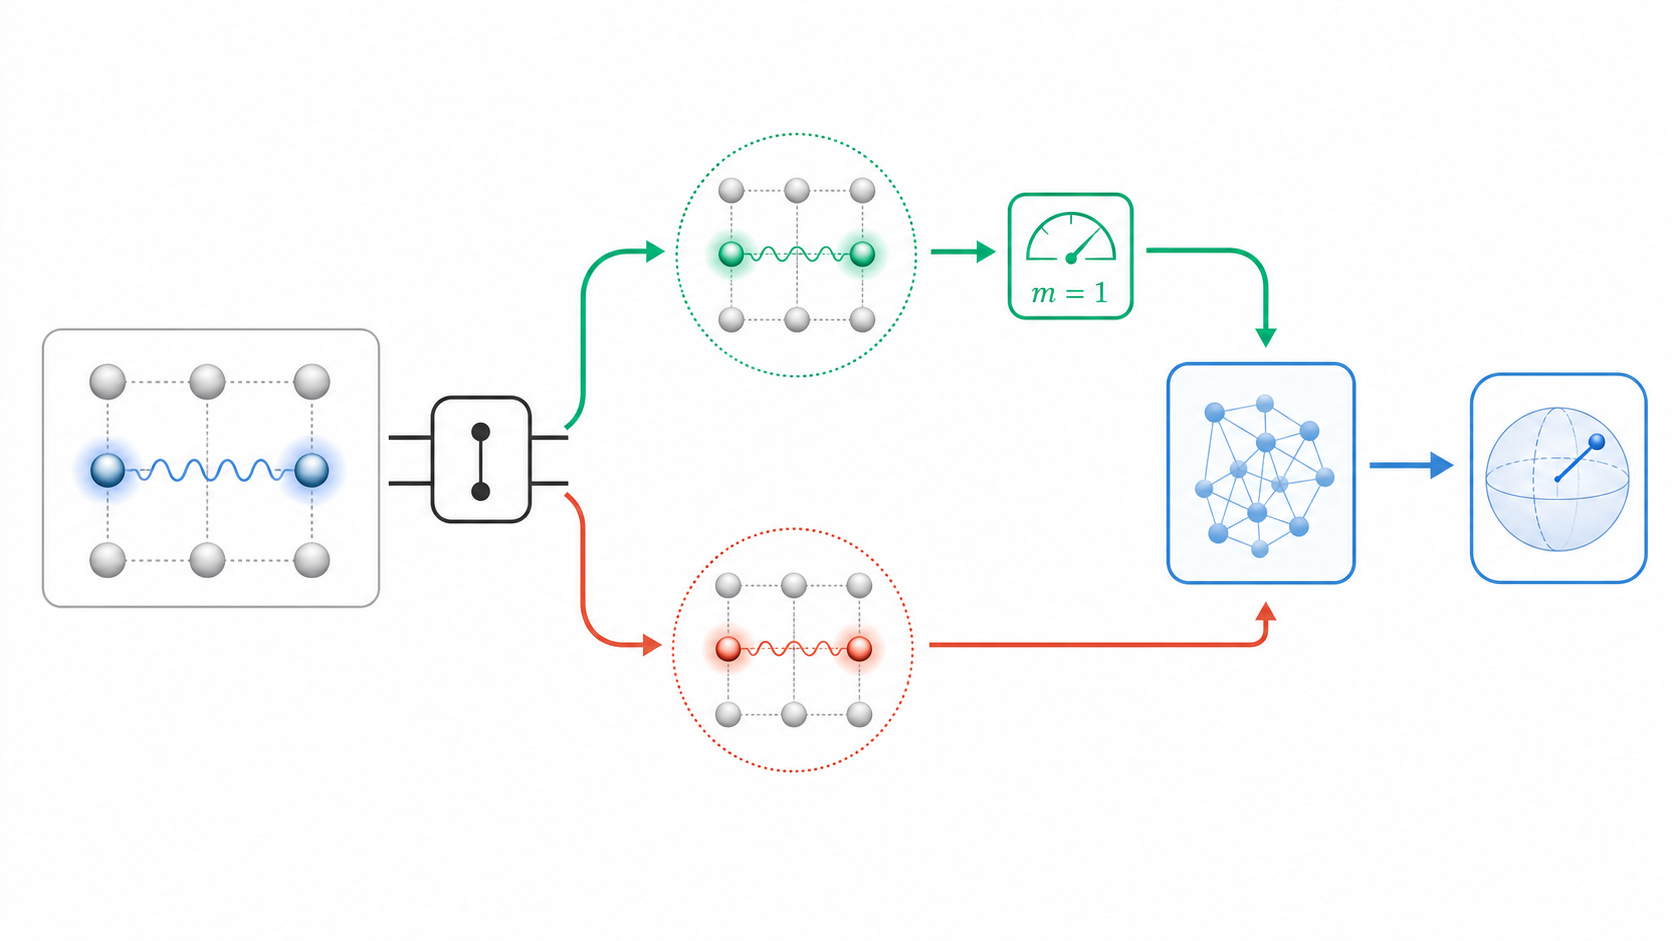
\includegraphics[height=0.49\textheight]{figures/erasure_decoder_flow_imagegen.png}
  \end{center}

  \vspace{-2mm}
  \begin{block}{Main point}
    A better Rydberg gate for logical qubits is not only a higher-fidelity
    gate. It is a gate whose remaining errors are easier for the decoder to
    locate and use.
  \end{block}

\end{frame}

\begin{frame}{Three papers, one story}
  \small
  \begin{table}
    \centering
    \begin{tabular}{p{0.24\textwidth}p{0.30\textwidth}p{0.36\textwidth}}
      \toprule
      Paper & Role in the story & Takeaway for this talk \\
      \midrule
      Jandura--Thompson--Pupillo, PRX Quantum 2023
      \cite{janduraOptimizingRydbergGates2023}
      & Control objective for Rydberg gates
      & Optimize logical-qubit performance, not only Bell-state fidelity. \\
      Ma et al., Nature 2023
      \cite{maHighfidelityGatesMidcircuit2023a}
      & Physical erasure-conversion prototype
      & Metastable \(^{171}\mathrm{Yb}\) can turn part of gate error into a mid-circuit flag. \\
      Zhang et al., Nature Physics 2026
      \cite{zhangLogicalQubitsErasure2026}
      & Logical-qubit demonstration
      & Erasure checks, \([[4,2,2]]\) decoding, and adaptive execution close the hardware-to-logical loop. \\
      \bottomrule
    \end{tabular}
  \end{table}

  \[
    \text{robust control}
    \rightarrow
    \text{less unlocated error}
    \rightarrow
    \text{more useful erasure information}
    \rightarrow
    \text{better logical behavior}.
  \]
\end{frame}

\begin{frame}{Why fidelity alone misses the logical point}
  \begin{columns}[T,onlytextwidth]
    \begin{column}{0.47\textwidth}
      \begin{block}{Same total error}
        \[
          p_{\mathrm{tot}}=\pe+\pp .
        \]
        \[
          R_e=\frac{\pe}{\pe+\pp},
          \qquad
          \eta_e=\frac{1}{1-R_e}.
        \]
      \end{block}
    \end{column}
    \begin{column}{0.49\textwidth}
      \begin{block}{Different decoder input}
        \[
          \mathcal D:
          (s,\;m,\;\text{noise model})
          \longrightarrow R .
        \]
        Syndrome \(s\) says which checks fired. Erasure flags \(m\) say
        where a physical qubit left the computational subspace.
      \end{block}
    \end{column}
  \end{columns}

  \vspace{3mm}
  \begin{center}
    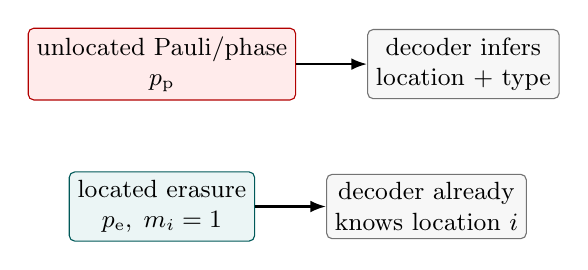
\begin{tikzpicture}[node distance=9mm]
      \node[smallbox, bad] (p) {unlocated Pauli/phase\\\(\pp\)};
      \node[smallbox, neutral, right=of p] (infer) {decoder infers\\location + type};
      \node[smallbox, good, below=of p] (e) {located erasure\\\(\pe,\;m_i=1\)};
      \node[smallbox, neutral, right=of e] (known) {decoder already\\knows location \(i\)};
      \draw[arrow] (p) -- (infer);
      \draw[arrow] (e) -- (known);
    \end{tikzpicture}
  \end{center}
\end{frame}

\begin{frame}{Physical story: leakage becomes a correctable erasure}
  \begin{columns}[c,onlytextwidth]
    \begin{column}{0.53\textwidth}
      \centering
      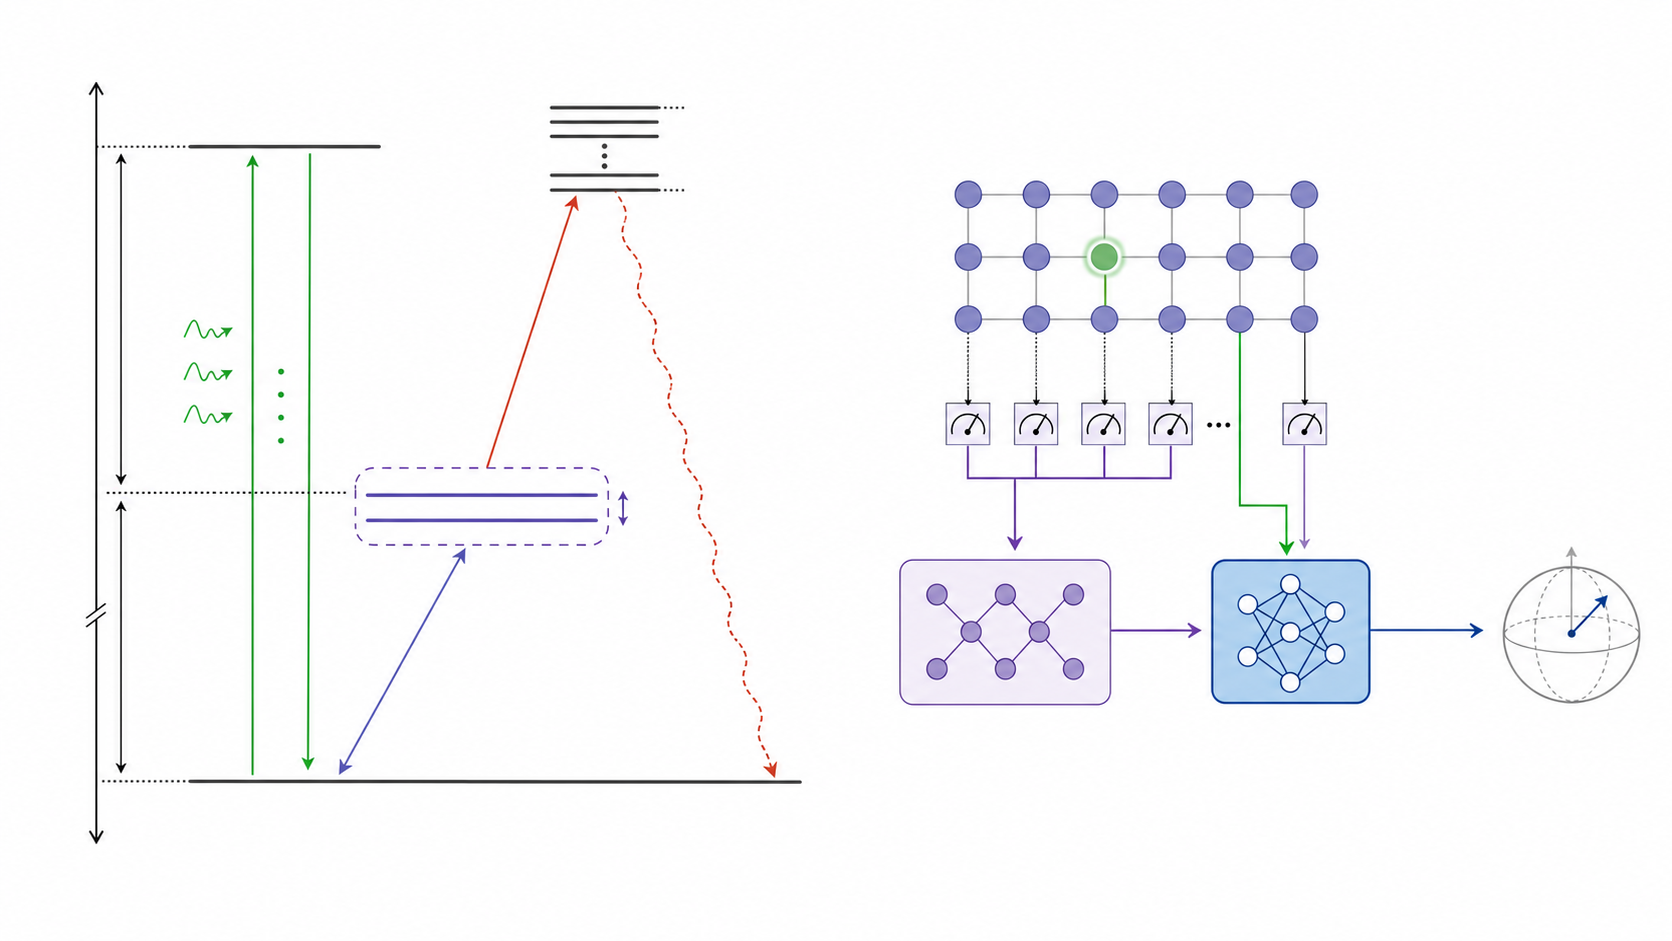
\includegraphics[width=0.98\textwidth]{figures/yb171_erasure_levels_qec_imagegen.png}
    \end{column}
    \begin{column}{0.44\textwidth}
      \scriptsize
      \setlength{\abovedisplayskip}{2pt}
      \setlength{\belowdisplayskip}{2pt}

      \textbf{Level structure.}
      \[
        \ket0,\ket1\subset{}^{3}P_0,
        \qquad
        \C=\mathrm{span}\{\ket0,\ket1\}.
      \]
      Leakage or decay can move population to \(^{1}S_0\).

      \vspace{1.2mm}
      \textbf{Erasure conversion.}
      \(399\,\mathrm{nm}\) imaging drives the cycling transition
      \(^{1}S_0\leftrightarrow{}^{1}P_1\):
      \[
        {}^{1}S_0\Rightarrow \text{bright}\Rightarrow m_i=1,
        \qquad
        {}^{3}P_0\Rightarrow \text{dark}.
      \]

      \vspace{1.2mm}
      \textbf{QEC use.}
      \[
        (s,\;m_i=1,\;\text{noise model})
        \xrightarrow{\mathcal D} R_i .
      \]
      The decoder knows the damaged location, so this leakage is treated
      as a located erasure rather than an unknown Pauli error.
    \end{column}
  \end{columns}
\end{frame}

\begin{frame}{Erasure conversion hardware: metastable \texorpdfstring{\(^{171}\mathrm{Yb}\)}{171Yb}}
  \begin{columns}[T,onlytextwidth]
    \begin{column}{0.56\textwidth}
      \centering
      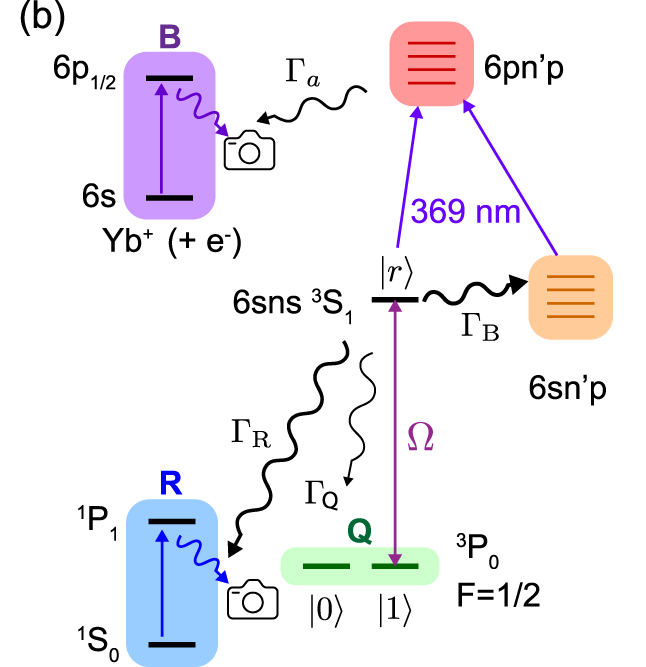
\includegraphics[height=0.72\textheight]{figures/wu2022_fig1b_erasure_conversion.png}
    \end{column}
    \begin{column}{0.41\textwidth}
      \small
      \textbf{What the figure contributes}
      \begin{itemize}
        \item Qubits are the two \(m_F\) states in metastable \(^{3}P_0\).
        \item Rydberg gates drive \(\ket1\leftrightarrow\ket r\) at \(302\,\mathrm{nm}\).
        \item Decay mostly leaves \(\C\): radiative \(R\), blackbody \(B\), or small return \(Q\).
        \item \(R\) and \(B\) can be detected without disturbing dark \(^{3}P_0\) qubits.
      \end{itemize}

      \[
        \mathcal H
        =
        \C_{3P0}
        \oplus
        \E_{1S0}
        \oplus
        \mathcal L_{\mathrm{other}}
        \oplus
        \mathcal A_{\mathrm{loss}} .
      \]
    \end{column}
  \end{columns}

  \vspace{1mm}
  {\scriptsize Source image: Wu et al. 2022, cropped Fig. 1b, Nature Communications \cite{wuErasureConversionFaulttolerant2022}.}
\end{frame}

\begin{frame}{QEC layer: the \texorpdfstring{\([[4,2,2]]\)}{[[4,2,2]]} code uses erasure locations}
  \begin{columns}[T,onlytextwidth]
    \begin{column}{0.57\textwidth}
      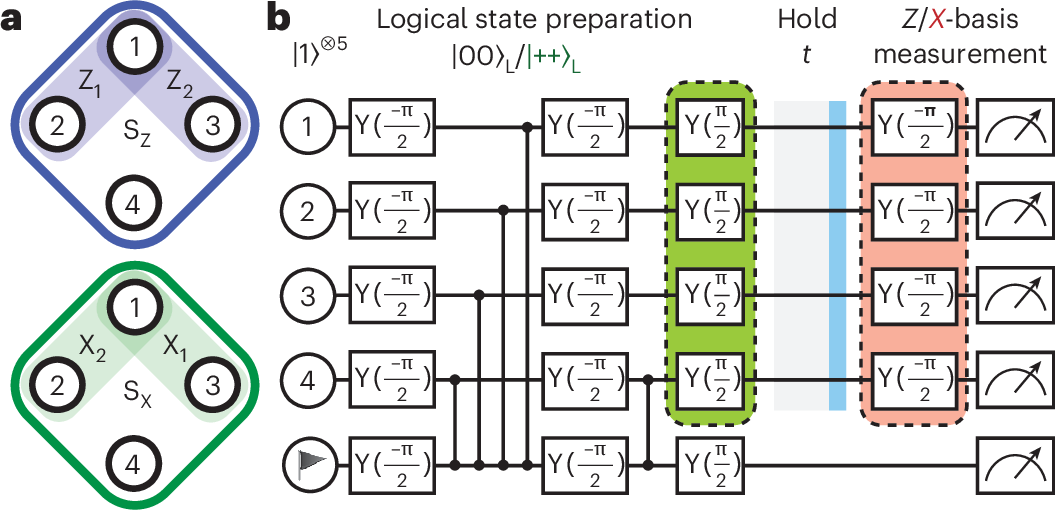
\includegraphics[width=\textwidth]{figures/zhang2026_fig3ab_422_code.png}
    \end{column}
    \begin{column}{0.40\textwidth}
      \small
      Stabilizers:
      \[
        S_Z=Z_1Z_2Z_3Z_4,
        \qquad
        S_X=X_1X_2X_3X_4 .
      \]

      Distance \(d=2\) means:
      \[
        \left\lfloor\frac{d-1}{2}\right\rfloor=0
      \]
      unknown Pauli errors are not generally correctable.

      \vspace{2mm}
      But one known-location erasure is usable:
      \[
        (s,\;i_{\mathrm{erased}})
        \Rightarrow
        \text{conditional decoding}.
      \]
    \end{column}
  \end{columns}

  \vspace{1mm}
  {\scriptsize Source image: Zhang et al. 2026, cropped Fig. 3a,b \cite{zhangLogicalQubitsErasure2026}.}
\end{frame}

\begin{frame}{Noise-robust control: where robust Rydberg pulses enter}
  \begin{columns}[T,onlytextwidth]
    \begin{column}{0.46\textwidth}
      \begin{block}{Physical channel split}
        \[
          \begin{aligned}
            \pe &= r\pd,\\
            \pp &\approx
            (1-r)\pd+(1-\pd)(1-\Fc).
          \end{aligned}
        \]
      \end{block}

      \small
      \(\pd\): Rydberg decay probability.

      \(\Fc\): fidelity conditioned on returning to \(\C\).

      \(r\): fraction of decay events converted into located erasure.
    \end{column}
    \begin{column}{0.50\textwidth}
      \begin{center}
        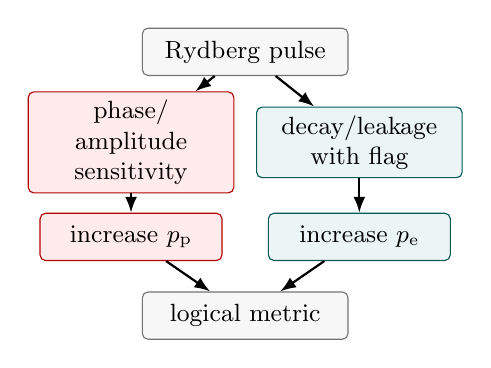
\begin{tikzpicture}[x=1cm,y=1cm]
          \node[smallbox, neutral, text width=24mm] (pulse) at (0,0) {Rydberg pulse};
          \node[smallbox, bad, text width=24mm] (phase) at (-1.45,-1.15) {phase/\\amplitude\\sensitivity};
          \node[smallbox, good, text width=24mm] (decay) at (1.45,-1.15) {decay/leakage\\with flag};
          \node[smallbox, bad, text width=21mm] (pp) at (-1.45,-2.35) {increase \(\pp\)};
          \node[smallbox, good, text width=21mm] (pe) at (1.45,-2.35) {increase \(\pe\)};
          \node[smallbox, neutral, text width=24mm] (logical) at (0,-3.35) {logical metric};
          \draw[arrow] (pulse) -- (phase);
          \draw[arrow] (pulse) -- (decay);
          \draw[arrow] (phase) -- (pp);
          \draw[arrow] (decay) -- (pe);
          \draw[arrow] (pp) -- (logical);
          \draw[arrow] (pe) -- (logical);
        \end{tikzpicture}
      \end{center}
    \end{column}
  \end{columns}

  \vspace{2mm}
  \begin{block}{Control objective}
    Robust pulses can accept some extra Rydberg exposure if they suppress
    no-flag computational-subspace sensitivity.
  \end{block}
\end{frame}

\begin{frame}{How AR, DR, and ADR pulses are generated}
  \scriptsize
  \setlength{\abovedisplayskip}{2pt}
  \setlength{\belowdisplayskip}{2pt}
  \begin{columns}[T,onlytextwidth]
    \begin{column}{0.48\textwidth}
      \textbf{Shared GRAPE setup.}
      The resonant blockade CZ is written as a piecewise pulse
      \(\Omega(t)=|\Omega_k|e^{i\phi_k}\). For each computational branch
      \(q\in\{01,10,11\}\),
      \[
        \ket{\psi_q(\tau)}
        =
        \ket{\psi_q^{(0)}(\tau)}
        +\sum_\alpha \lambda_\alpha
        \ket{\psi_{q,\alpha}^{(1)}(\tau)}
        +O(\lambda^2).
      \]
      The zero-order trajectory must close and accumulate the CZ phase.

      \vspace{1mm}
      \textbf{AR: amplitude robust.}
      \(\lambda_\alpha=\epsilon_i\) rescales the Rabi coupling. Since
      \(\epsilon_i\) does not reverse in a second half, the pulse itself must
      remove first-order response:
      \[
        J_{\mathrm{AR}}
        =
        1-F+
        \sum_{q,i}
        \|\ket{\psi_{q,\epsilon_i}^{(1)}(\tau)}\|^2 .
      \]
    \end{column}

    \begin{column}{0.49\textwidth}
      \textbf{DR: Doppler robust.}
      Optimize a half pulse with half the entangling phase. Doppler shifts
      \(\Delta_i=k v_i\) are reversed between halves by
      \(k\rightarrow-k\) or by waiting half a trap period:
      \[
        (I-\ket q\!\langle q|)
        \ket{\psi_{q,\Delta_i}^{(1)}(\tau_h)}=0 .
      \]
      Longitudinal first-order phases are allowed because they cancel after
      the sign-reversed second half.

      \vspace{1mm}
      \textbf{ADR: amplitude and Doppler robust.}
      The same half-pulse variables satisfy both constraints:
      \[
        J_{\mathrm{ADR}}
        =
        1-F_h+
        J_{\epsilon}^{(1)}
        +J_{\Delta,\perp}^{(1)} .
      \]
      It is not an AR pulse concatenated with a DR pulse; the constraints
      compete on one trajectory.
    \end{column}
  \end{columns}

  \vspace{1mm}
  \begin{center}
    \scriptsize
    Cost of robustness:
    \(\tau_R^{\mathrm{TO}}=2.96\),
    \(\tau_R^{\mathrm{AR}}=4.74\),
    \(\tau_R^{\mathrm{DR}}=5.56\),
    \(\tau_R^{\mathrm{ADR}}=10.37\)
    in units of \(1/\Omega_{\max}\)
    \cite{janduraOptimizingRydbergGates2023}.
  \end{center}
\end{frame}

\begin{frame}{Robust-pulse result: flatter response to technical noise}
  \centering
  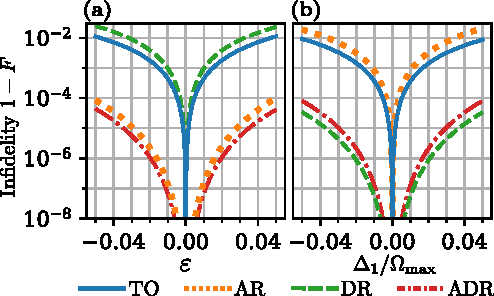
\includegraphics[width=0.88\textwidth,height=0.58\textheight,keepaspectratio]{figures/jandura2023_fig2ab_robustness.pdf}

  \vspace{1mm}
  \begin{columns}[T,onlytextwidth]
    \begin{column}{0.48\textwidth}
      \scriptsize
      \textbf{Amplitude noise.}
      AR and ADR flatten \(1-F\) versus common Rabi-amplitude error
      \(\epsilon\); TO and DR remain amplitude sensitive.
    \end{column}
    \begin{column}{0.48\textwidth}
      \scriptsize
      \textbf{Doppler noise.}
      DR and ADR flatten \(1-F\) versus \(\Delta_1/\Omega_{\max}\);
      ADR is the joint robust choice when both noise sources matter.
    \end{column}
  \end{columns}

  \vspace{0.5mm}
  {\scriptsize Source image: Jandura et al. 2023, cropped Fig. 2a,b, PRX Quantum \cite{janduraOptimizingRydbergGates2023}.}
\end{frame}

\begin{frame}{Overall result: erasure flags become useful logical information}
  \centering
  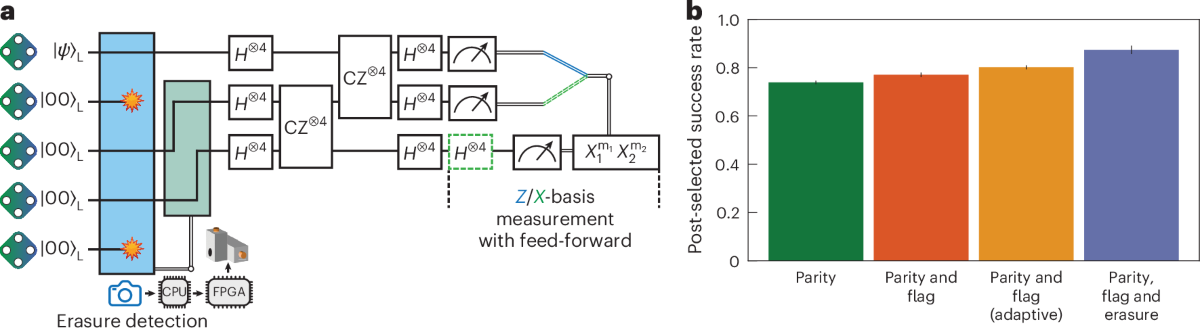
\includegraphics[width=\textwidth,height=0.58\textheight,keepaspectratio]{figures/zhang2026_fig4_teleportation.png}

  \vspace{1mm}
  \begin{columns}[T,onlytextwidth]
    \begin{column}{0.46\textwidth}
      \scriptsize
      \textbf{Protocol ladder.}
      The experiment compares parity-only operation, adding flag information,
      adaptive feed-forward, and finally adaptive decoding with erasure records.
    \end{column}
    \begin{column}{0.50\textwidth}
      \scriptsize
      \textbf{Main effect.}
      The post-selected success rate increases across this ladder, showing that
      erasure conversion is not only a diagnostic: it supplies location
      information that can be used during logical execution.
    \end{column}
  \end{columns}

  \vspace{0.5mm}
  {\scriptsize Source image: Zhang et al. 2026, Fig. 4, Nature Physics \cite{zhangLogicalQubitsErasure2026}.}
\end{frame}

\begin{frame}{The deck's compressed takeaway}
  \begin{enumerate}
    \item The logical layer cares about the pair \((\pe,\pp)\), not only \(\pe+\pp\).
    \item Metastable \(^{171}\mathrm{Yb}\) gives a useful physical interface:
      qubits are dark, some leakage/decay is bright.
    \item \([[4,2,2]]\) is intentionally small: it makes the value of one known
      erased location visible.
    \item Adaptive logical circuits are the real milestone: erasure flags are
      used during execution, not only after the experiment.
    \item For this repository, the natural next simulation target is an
      erasure-aware physical-to-logical score for shaped \(^{171}\mathrm{Yb}\)
      CZ pulses.
  \end{enumerate}
\end{frame}

\begin{frame}[allowframebreaks]{References}
  \printbibliography
\end{frame}

\end{document}
